\begin{frame}{Aufgabe 1}{Struktogramm}
Auf der folgenden Folie wird ein Algorithmus durch ein Struktogramm beschrieben. Übergeben wird eine ganzzahlige Zahl \texttt{n}
\begin{enumerate}
    \item Bestimmt $O$
    \item Welche Aufgabe hat der Algorithmus
    \item Ist der Algorithmus korrekt?
    \begin{itemize}
        \item Wenn nicht, nennt ein Beispiel für \texttt{n}, in dem der Algorithmus fehlschlägt
    \end{itemize}
\end{enumerate}
\end{frame}

\begin{frame}{Aufgabe 1}{Struktogramm}
\begin{centernss}
    \begin{struktogramm}(70,60)
        \assign{Lese \( n \) ein}
        \assign{Setze \( res \) auf \( 1 \) }
        \until{n!=0}
            \assign{\( res = res*n\)}
            \assign{\( n-- \)}
        \untilend
        \assign{Gib \( res \) aus}
    \end{struktogramm}
\end{centernss}
\end{frame}

\begin{frame}{Aufgabe 2}{Größter Teiler}
Entwerft einen Algorithmus, der für einen gegebene natürliche Zahl den größten (ganzzahligen) Teiler findet. Erstellt zu eurem Algorithmus einen Programmablaufplan oder Struktogramm.

Analysiert euren Algorithmus bezüglich der Komplexität $O$. Vergleicht euren Algorithmus mit denen der anderen.
\end{frame}

\begin{frame}[fragile]{Aufgabe 3}{Codeanalyse}
Analysiert den folgenden Codeausschnitt. Welche Aufgabe hat der Algorithmus? Bestimmt die Komplexität $\tau(4,2)$, $\tau(N,M)$ und $O$.

Hinweis: $N$ bezeichnet hierbei die Länge der Liste \texttt{in1} und $M$ die Länge der Liste \texttt{in2}

\lstset{style=java}
\begin{lstlisting}
public void func(List<?> in1, List<?> in2){
  for(int i=0;i<in1.size();i++){
      for(int j=0;in2.size();j++){
          String out = String.format("{\%s,\%s}", in1.get(i), in2.get(j));
          System.out.println(out);
      }
  }
}
\end{lstlisting}
\end{frame}

\begin{frame}{Aufgabe 4}{Programmablaufplan}
Auf der folgenden Folie findet Ihr einen Algorithmus in Form eines Programmablaufplans. 
\begin{enumerate}
    \item Was ist der Ziel des Algorithmus?
    \item Bestimmt $\tau(n)$ und $O(n)$.
    \item Lässt sich der Algorithmus noch verbessern in Blick auf die Effizienz?
    \begin{itemize}
        \item Wenn ja, wie?
        \item Wenn ja, bestimmt für die Optimierung $\tau(n)$ und $O(n)$
    \end{itemize}
    \item Implementiert den Algorithmus (In Java oder einer Sprache eurer Wahl)
\end{enumerate}
\end{frame}

\begin{frame}{Aufgabe 4}{Programmablaufplan}
\begin{figure}
    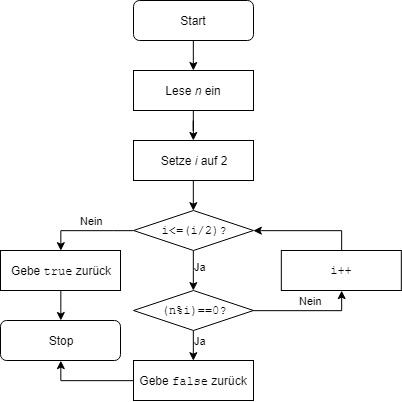
\includegraphics[height=5cm]{graph/pap_excercise_algo}
\end{figure}
\end{frame}

\begin{frame}{Aufgabe 5}{Best- und Worst-Case Execution Time}
Auf der folgenden Folie findet ihr einen Codeausschnitt mit variabler Komplexität.

\begin{enumerate}
    \item Bestimme $\tau(N)$ für den Best- und Worst-Case.
    \item Unter welchen Bedingungen tritt der Best- bzw. Worst-Case ein?
    \item Bestimme $O$
\end{enumerate}
\end{frame}

\begin{frame}[fragile]{Aufgabe 5}{Best- und Worst-Case Execution Time}
\lstset{style=java}
\begin{lstlisting}
public void func(int[] array, int n){
    for(int i=0;i<n;i++){
        if((array[i]%2)==0){
            array[i]+=1;
            array[i]*=7;
            array[i]*=array[i];
            array[i]-=42;
            array[0]+=array[i];
        }else{
            array[i]+=2;
        }
    }
}
\end{lstlisting}
\end{frame}